\section{Introduction}

The results of a Bayesian multivariate classifier are presented.
An explanation of its development is provided.
The classifier was trained to work with three categories $C_i$ and a
feature vector of size 2.

The classifier was trained using the Iris flower data set
\cite{fisher1936iris}, available from the UCI Machine
Learning Repository \footnote{https://archive.ics.uci.edu/ml/datasets/Iris}.
The dataset describes five properties of three different flower species:
petal length, petal width, sepal length, sepal width and variety.
Whilst the first four are quantitative traits, the last one is qualitative.
This trait describes the type flower associated with the entry:
Iris setosa, Iris versicolor and Iris virginica.
Figure \ref{fig: iris} presents the species in the dataset.


\begin{figure}[htb!]
    \centering
    \begin{subfigure}[b]{0.3\textwidth}
        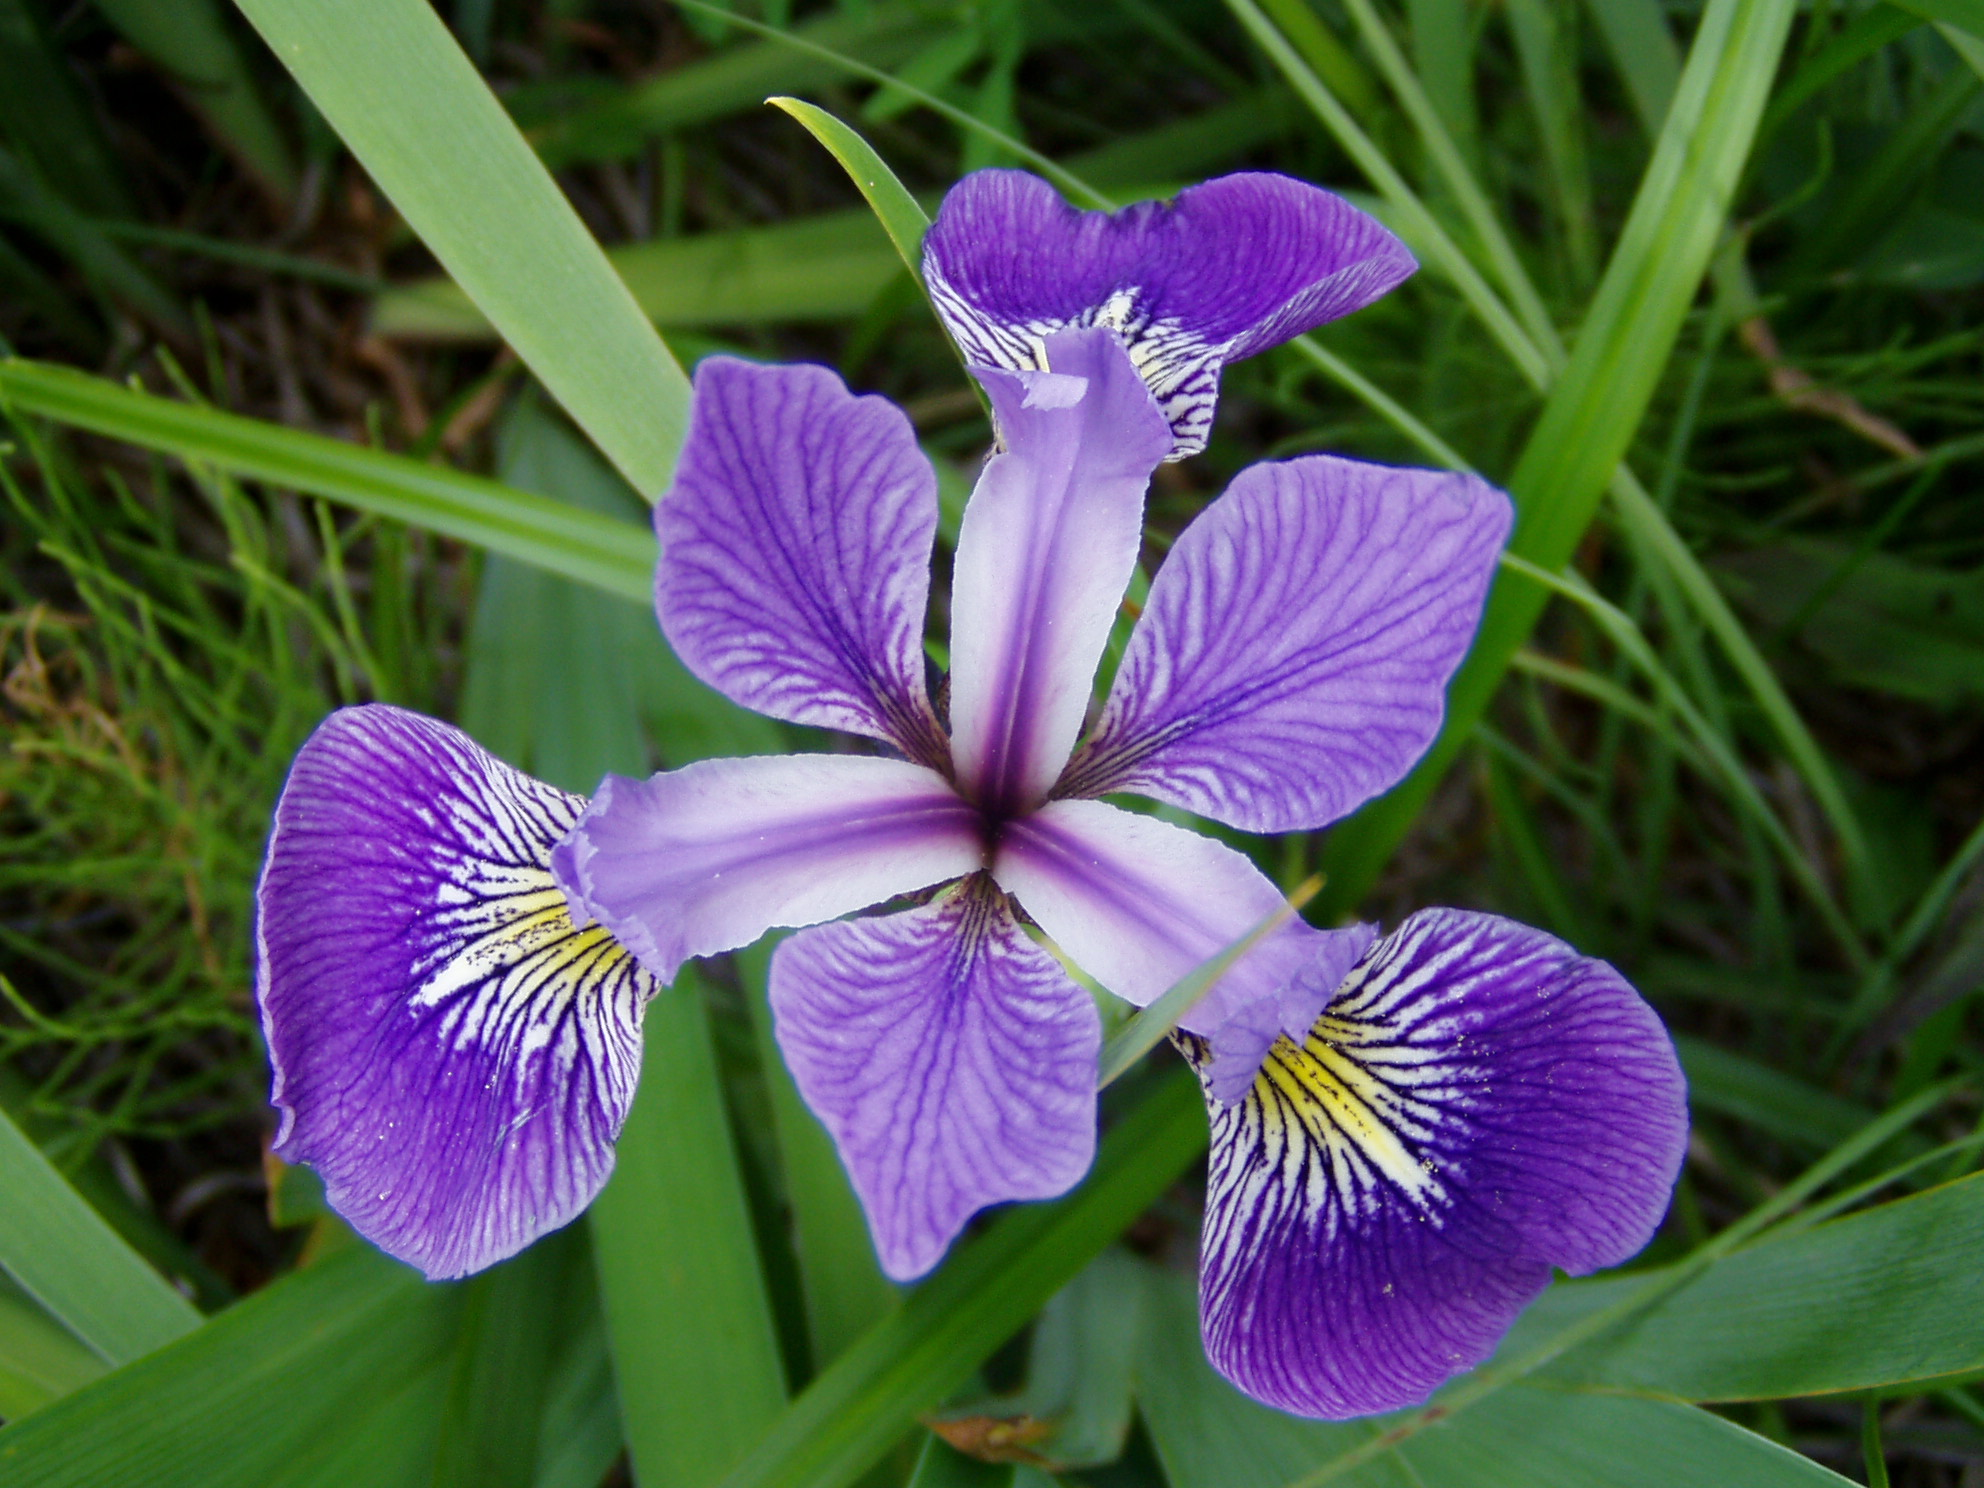
\includegraphics[width=\textwidth]{Iris_versicolor_3}
        \caption{Iris versicolor}
        \label{fig: versicolor}
    \end{subfigure}
    ~ %add desired spacing between images, e. g. ~, \quad, \qquad, \hfill etc.
      %(or a blank line to force the subfigure onto a new line)
    \begin{subfigure}[b]{0.3\textwidth}
        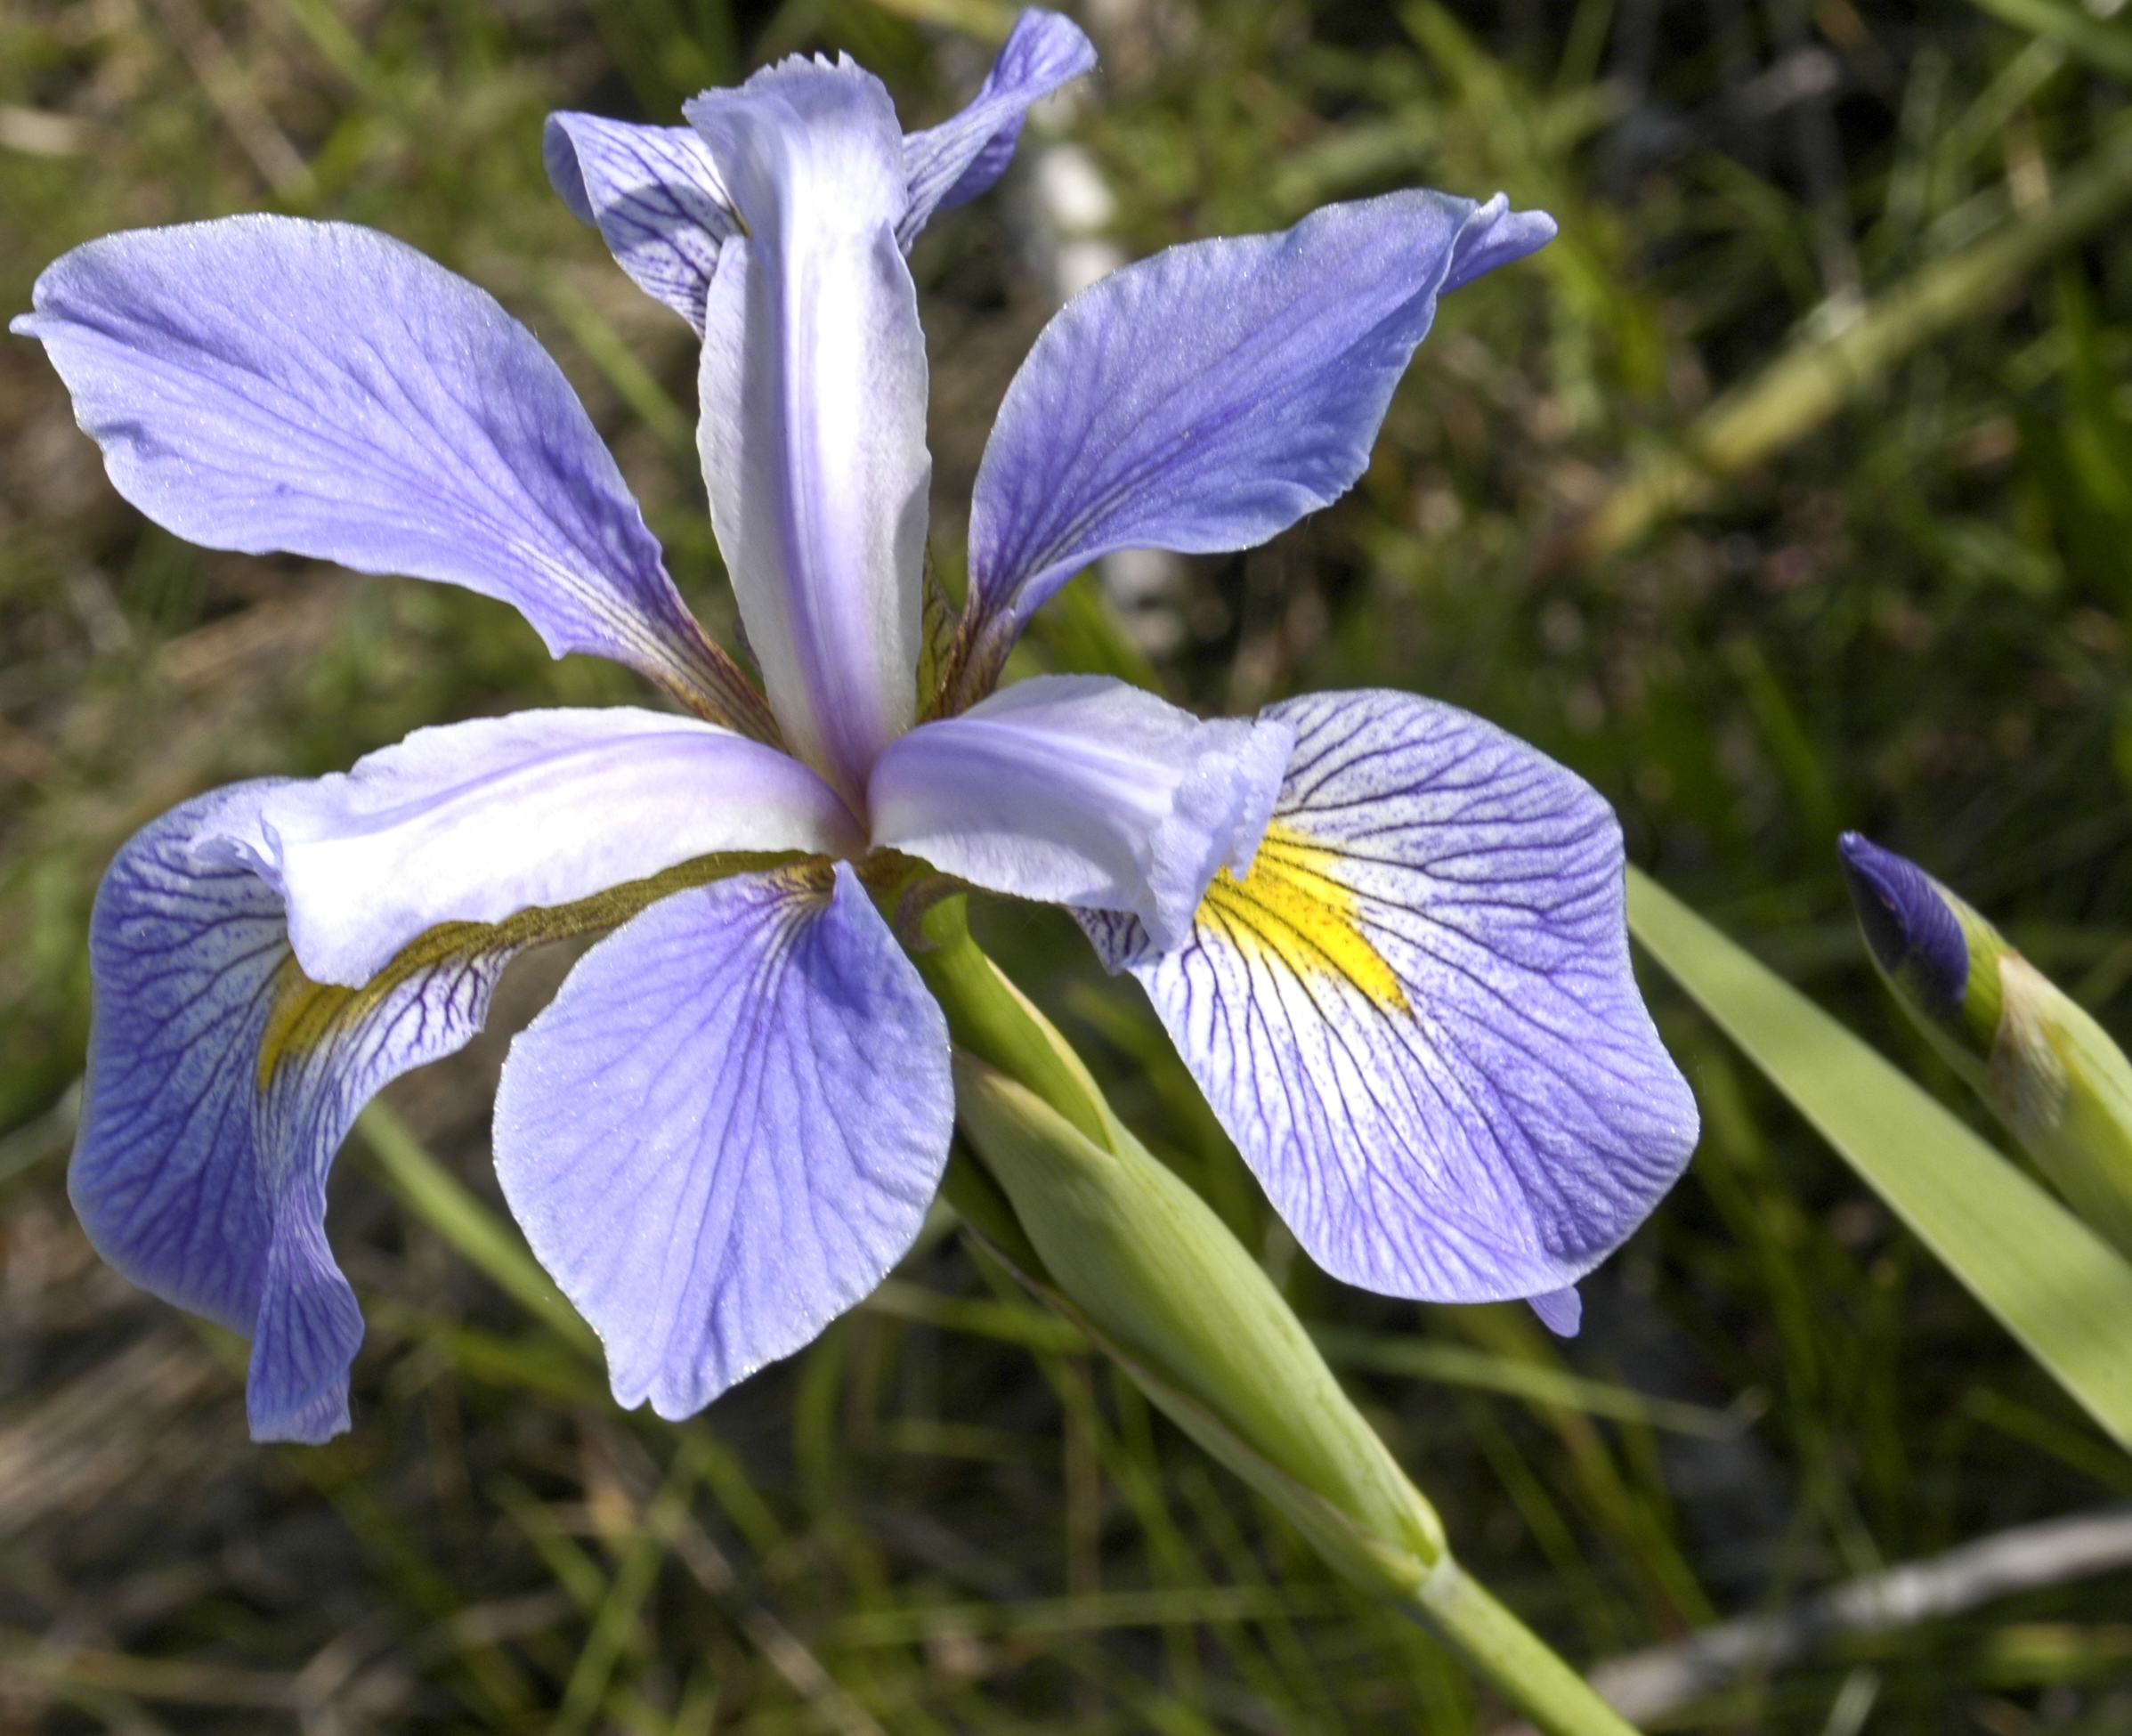
\includegraphics[width=\textwidth]{Iris_virginica}
        \caption{Iris virginica}
        \label{fig: virginica}
    \end{subfigure}
    ~ %add desired spacing between images, e. g. ~, \quad, \qquad, \hfill etc.
    %(or a blank line to force the subfigure onto a new line)
    \begin{subfigure}[b]{0.3\textwidth}
        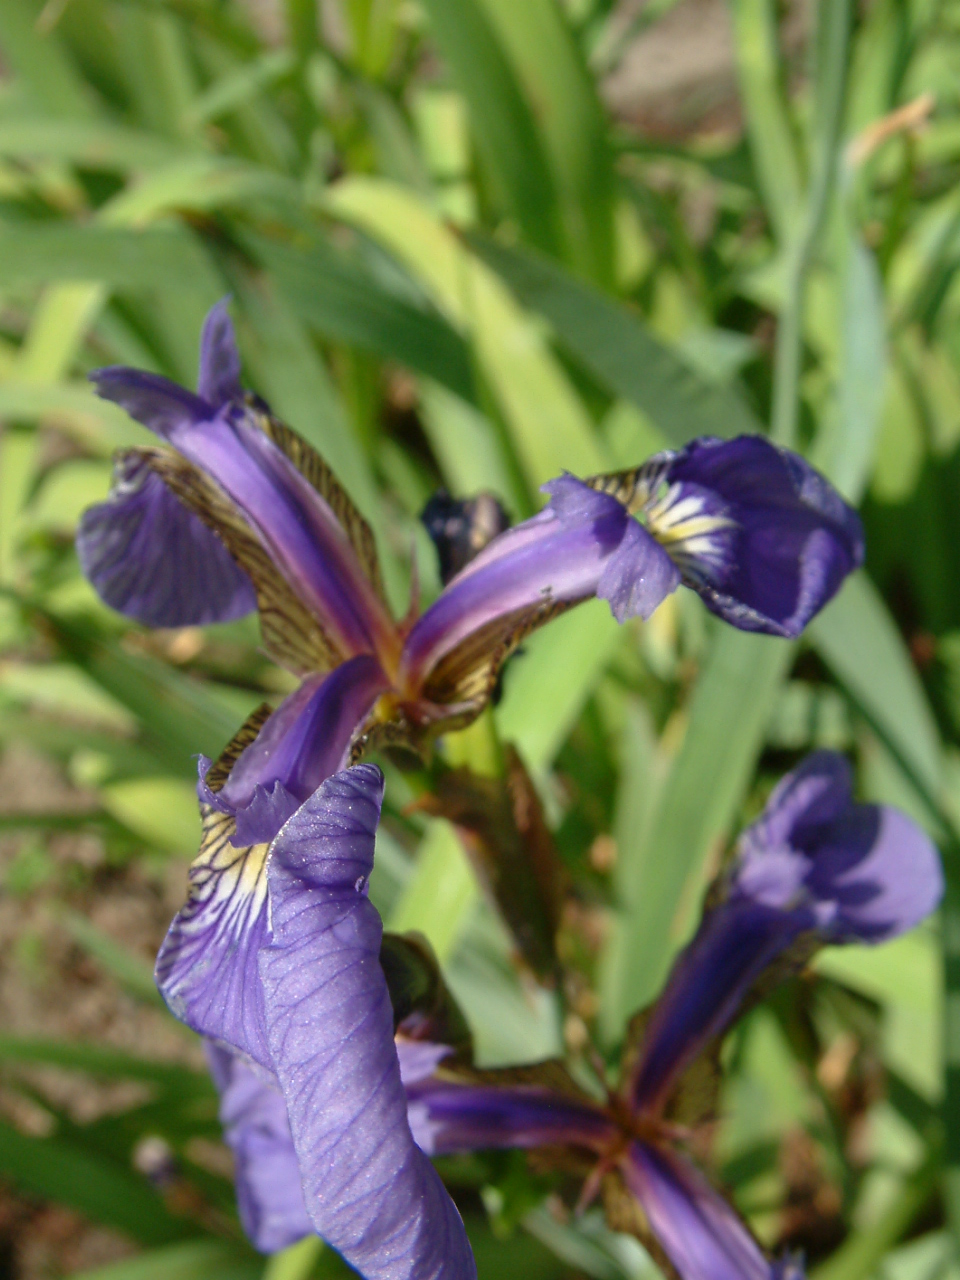
\includegraphics[width=\textwidth]{Kosaciec_szczecinkowaty_Iris_setosa}
        \caption{Iris setosa}
        \label{fig: setosa}
    \end{subfigure}
    \caption{Species in the iris dataset}\label{fig: iris}
\end{figure}

\section{Features in the data set}

From the data set, two groups of features are identified: length and width for petal and sepal.
To develop a classifier of size two, it is necessary to select the two entries from the feature vector
that will be used in the classifier.
Observing the grouping of datapoints for length and width
(Figure \ref{fig: dataset}) it becomes evident that the petal traits are ideal for the classifier.
This is due to how the data is already grouped into three easily identifiable groups.

\begin{figure}[htb!]
\centering
 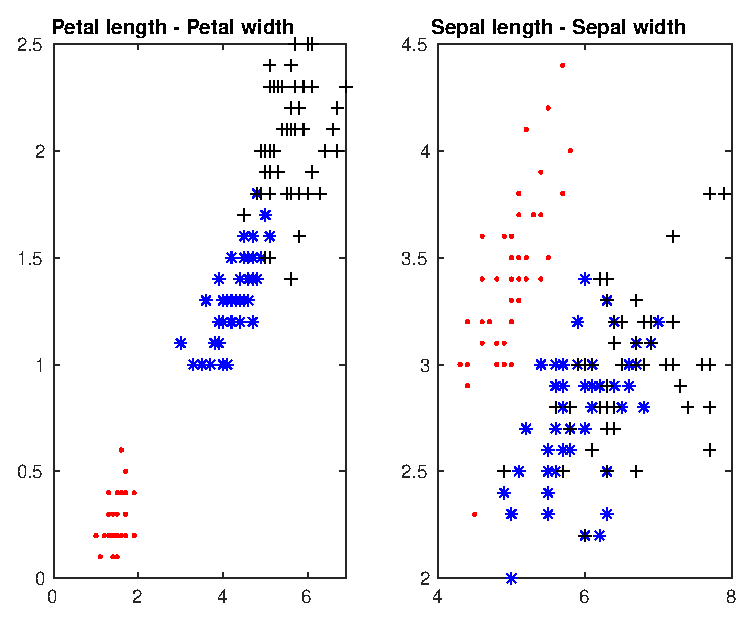
\includegraphics[width=\textwidth]{dataset}
 \caption{Data clusters}
 \label{fig: dataset}
\end{figure}

